\chapter{The ATLAS Detector}

The \ac{ATLAS} detector is a cylindrical general purpose particle detector designed to measure the products of $\sqrt{s} = 14 \TeV$ proton-proton collisions at the \ac{LHC}. It consists of three major sub-detectors: closest to the beamline is the the \ac{ID}, which measures the trajectories of charge particles, followed by the Calorimeters, which measure the energies of electromagnetic and hadronically interacting particles, and finally the \ac{MS} which measures the trajectories of muons. The \ac{ID} is surrounded by a super conducting solenoidal magnet that provides a uniform $2\textrm{T}$ magnetic field, enabling measurement of particles' charge and momentum, and a toroidal magnet surrounds \ac{MS}, allowing for charge and momentum measurements of muons. In general, each subdetector consists of a barrel detector parallel to the beampipe and end-cap detectors perpendicular to the beampipe. \cite{atlas-overview}

A schematic of the \ac{ATLAS} detector is shown in \autoref{fig:atlas-schematic}.


%https://atlas.cern/discover/detector
\begin{figure}[htbp]
\centering
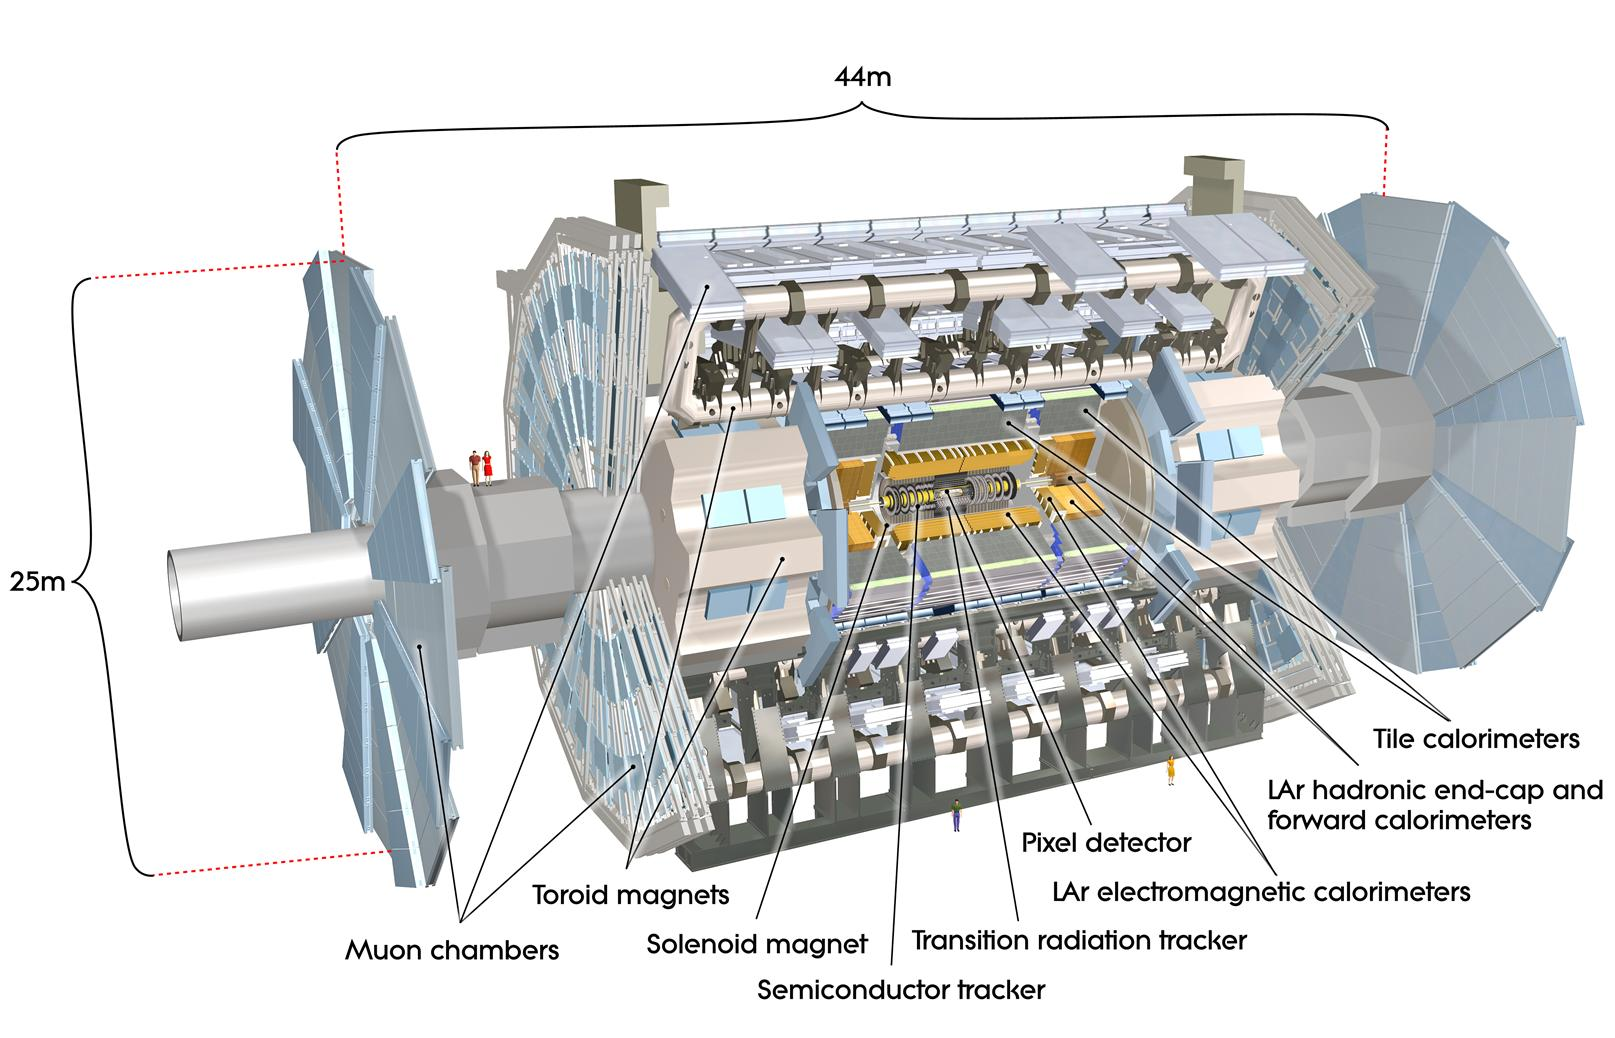
\includegraphics[width=.8\textwidth]{figures/Detector/atlas-schematic.jpg}
\caption{A diagram of the \ac{ATLAS} detector. The dimensions, subdetectors, and magnet systems are labeled. }
\label{fig:atlas-schematic}
\end{figure}

\section{Coordinate System}
\ac{ATLAS} uses a Cartesian right-handed coordinate system, with the origin defined as the $pp$ collision point. The $z$-axis points along the beampipe, where $+z$ points counter-clockwise. The transverse plane, the $y$-axis and $x$-axis, points upward and toward the center of the \ac{LHC} ring, respectively. The detector is built with with symmetry across the origin in in $z$, as well as with rotational symmetry in the transverse plane. The $+z$ side of the detector is referred to as the A-side, and $-z$ as the C-side.

Cylindrical coordinates provide a comfortable description of the \ac{ATLAS} detector, where $\phi$ measures the angle in the $x-y$ plane around the beampipe, and $\theta$ the angle from the $z$ axis. $\phi$ is positive for positive $y$. 

A given particle's momentum in $z$ is not known, but its transverse momentum is known to be $0$, so it is advantageous to define spatial variables independent of $z$ momentum. Thus, instead of $\theta$, $\eta = - \textrm{ln}(\textrm{tan}\frac{\theta}{2})$ is used to describe angle from the $z$ axis. Particles perpendicular to the $z$ axis have $\eta = 0$, while those parallel to the beamline have $\eta \rightarrow \infty$. 

Angular distances between objects is described using $\Delta R = \sqrt{\Delta \eta ^2 + \Delta \phi ^2}$ and the radial distance from the origin in the $x-y$ plane is denoted $R$. 

A particle's momentum will generally be described in terms of its \pT, its momentum in the transverse direction. A particle's $3$-vector is described by $(\pt, \eta, \phi)$, which are all invariant under boosts in $z$ assuming the particle can be considered massless (which is true in the case of particles in \ac{ATLAS}).





%USED ATLAS-overview.pdf
\section{Inner Detector}
The Inner Detector measures the trajectories of charged particles resulting from \ac{LHC} collisions. The \ac{ID} covers the region with $|\eta| < 2.5$, measuring approximately $1000$ particles per bunch crossing. In order to achieve the momentum and vertex resolution required to achieve \ac{ATLAS}'s physics goals three subdetectors are used: the Pixel detector, the \ac{SCT}, and the \ac{TRT}. The Pixel and \ac{SCT} detectors are used for high granularity precision tracking and the \ac{TRT} is used to distinguish electrons from converted photons. All of this is immersed in a $2T$ magnetic field, curving charged particles in proportion to its momentum.

\todo{describe conversions somewhere... Maybe in particle descriptions in theory?}


The \pt resolution of the \ac{ID} scales with track \pt. Higher \pt tracks are less curved, so the measurement resolution is worse. In the \ac{ATLAS} \ac{ID}, the \pt resolution  $0.05\% \times \pt$ with a $1\%$ constant term. The constant term describes measurement uncertainties that do not scale with momentum or energy, such as material imperfections, non-uniform detector response, or other constant measurement issues and is added in quadrature ($\oplus$) with the stochastic term.


A schematic of the \ac{ID} can be seen in \autoref{fig:atlas-id} and a detailed distribution of the various subdetectors is shown in \autoref{fig:atlas-id-layers}. 


%https://cds.cern.ch/images/CERN-GE-0803014-01/file?size=medium
\begin{figure}[htbp]
\centering
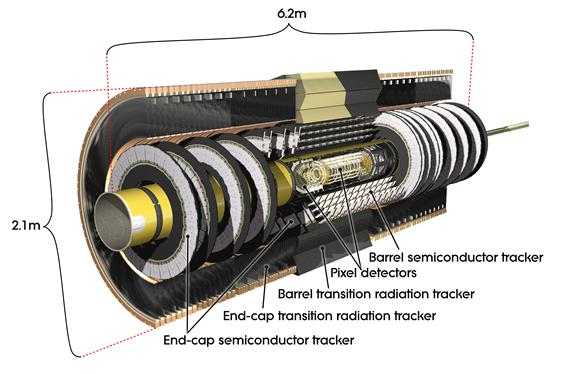
\includegraphics[width=.8\textwidth]{figures/Detector/atlas-ID.jpg}
\caption{A diagram of the \ac{ATLAS} \ac{ID} with the major subsystems labeled. The Pixel and \ac{SCT} are of particular importance for this analysis.}
\label{fig:atlas-id}
\end{figure}

%https://www.researchgate.net/publication/325643426/figure/fig8/AS:669532737769482@1536640452588/Segment-of-the-ATLAS-inner-detector-showing-the-tracker-layers-The-silicon-strip.ppm
\begin{figure}[htbp]
\centering
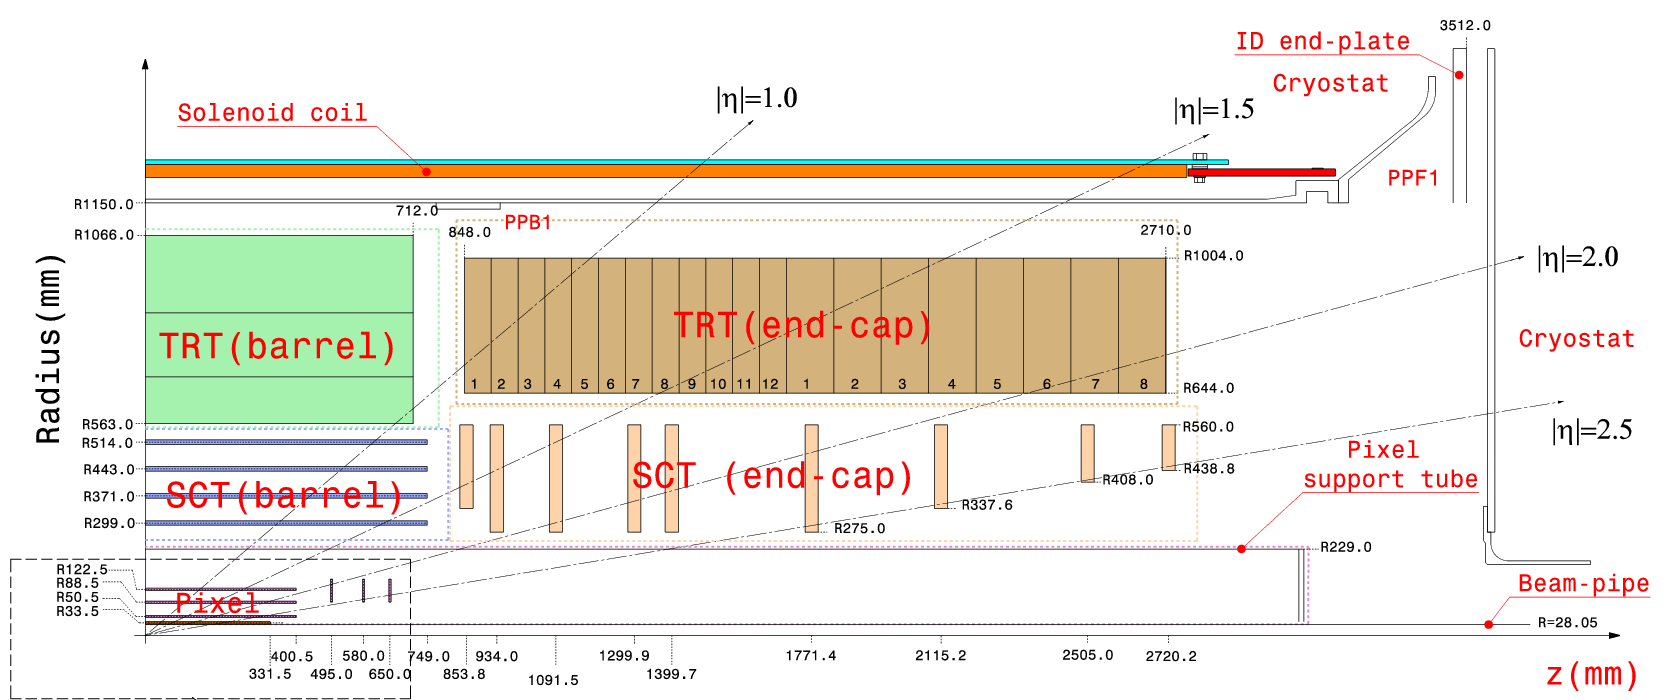
\includegraphics[width=.8\textwidth]{figures/Detector/atlas-id-layers.png}
\caption{A schematic of the \ac{ATLAS} \ac{ID} shown in the $r-z$ plane. \cite{id-cutaway}}
\label{fig:atlas-id-layers}
\end{figure}

\subsection{The Pixel Detector}
\subsubsection{Hit Reconstruction}
\subsection{The Silicon Microstrip Tracker}
\subsubsection{Hit Reconstruction}
\subsection{The Transition Radiation Tracker}

\subsection{Solenoid Magnet}

The central solenoid surrounds the \ac{ID} and provides a uniform $2\textrm{T}$ field that bends the trajectories of charged particles. The transverse momentum of the particle can be inferred from its radius of curvature, $R$, in the $x-y$ plane using the equation $p_{T} = qBR$, where $q$ is the charge of the particle and $B$ the magnetic field in the $z$ direction.

However, the placement of the solenoid between the \ac{ID} and calorimeters necessitates careful design choices so that all of a given particle's energy is still measured by the calorimeters. The solenoid only contributes about $0.66$ radiation lengths \footnote{Radiation lengths measure the mean distance in which an electron loses all but $\frac{1}{e}$ of its energy.}. In order to achieve this, the solenoid and \ac{EM} calorimeter share a vacuum vessel, eliminating the need for two vacuum walls. It is made of Al-stabilised NbTi superconductor which allows a high electric field to be achieved ($7.730 \textrm{kA}$) while optimizing the thickness of the coil. The solenoid has an axial length of $5.8 \textrm{m}$ and radial thickness of $100 \textrm{cm}$ and it operates at a temperature of $4.5 \textrm{K}$. 


\section{Calorimeters}

The \ac{ATLAS} calorimeters measure the energy of electromagnetic and hadronic particles. The calorimeter system is composed of \ac{EM}, hadronic, and forward calorimeters. While they use a variety of different technologies to measure energies, they are both sampling calorimeters composed of alternating active and absorbing layers. Particles shower in absorbing layers and the showers are measured in the active layers, but the actual energy of each particle is not measured because some is lost to the absorbing layers. Unlike the tracker, the energy resolution of a calorimeter increases with increasing energy due to the increased signal generated. The size of each calorimeter is set by its radiation length or nuclear interaction length such that the calorimeter absorbs all of given particle's energy by the far end of the calorimeter and only muons and neutrinos should escape the calorimeters layers. A schematic of the \ac{ATLAS} calorimeters can be seen in \autoref{fig:atlas-calos}


%https://arxiv.org/pdf/1603.02934.pdf
\begin{figure}[htbp]
\centering
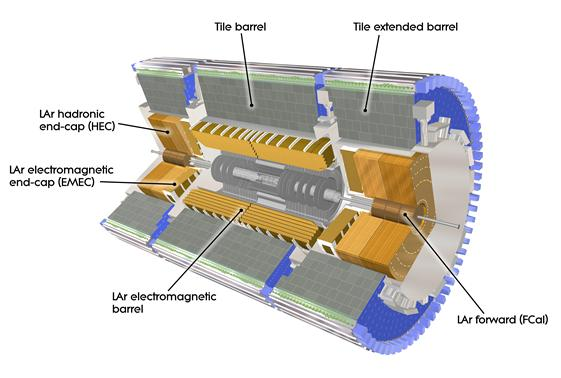
\includegraphics[width=.8\textwidth]{figures/Detector/atlas-calorimeters.jpg}
\caption{A diagram of the \ac{ATLAS} calorimeters with the major subsystems labeled. The \ac{EM} calorimeter is of particular importance for this analysis. \cite{calorimeters}}
\label{fig:atlas-calos}
\end{figure}


\subsection{Electromagnetic Calorimeter}

The \ac{LAr} \ac{EM} calorimeter is the innermost calorimeter and gives excellent energy and position resolution. \cite{calorimeters} It is composed of barrel ($|\eta| < 1.5$) and end-cap ($1.4 < |\eta| < 3.2$) components. Both components use a lead absorber with liquid argon active material. The layers of the calorimeter have an accordion shape (shown in \autoref{fig:atlas-lar}), which allows for the multiple absorbing layers without any gaps between them, as well as complete $\phi$ symmetry. The first layer has finer segmentation in $\eta$ to allow for more precise angular measurements of photons (which do not produce an \ac{ID} track). The thickness of the absorbing plates varies as a function of $\eta$ to optimize energy resolution. An active liquid argon presampler is placed before the accordion layers in the region with $|\eta| < 1.8$ to correct for energy loss upstream of the calorimeter. It is about 22 radiation lengths wide and gives energy resolution of $10\%/\sqrt{E} \oplus 0.7\%$

%https://www.researchgate.net/profile/Denis_Oliveira_Damazio/publication/229849719/figure/fig2/AS:667635272413188@1536188061121/Calorimeter-cells-for-different-layers-left-Note-the-very-fine-segmentation-in-the_Q320.jpg
\begin{figure}[htbp]
\centering
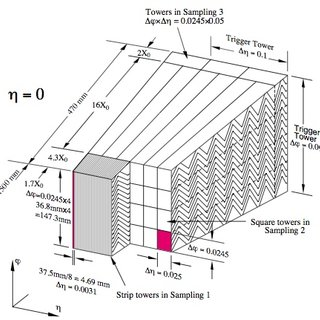
\includegraphics[width=.6\textwidth]{figures/Detector/lar.jpg}
\caption{A diagram of the \ac{ATLAS} \ac{EM} \ac{LAr} calorimeter. It has a unique shape in order to provide precision position and energy resolution.}
\label{fig:atlas-lar}
\end{figure}


\subsection{Hadronic Calorimeter}

The hadronic calorimeter surrounds the \ac{EM} calorimeter also within $|\eta| < 3.2$. The barrel region ($|\eta| < 1.7$) is made of steel absorbers with active material of scintillating tiles. Here, the calorimeter is about $2$m long in the radial direction and covers about $8$ interaction lengths. The Hadronic End-cap Calorimeters cover the region $1.5 < |\eta| < 3.2$ with a copper absorber and liquid argon active material.


The hadronic calorimeter has an energy resolution of  $50\%/\sqrt{E} \oplus 3\%$. 

\subsection{Forward Calorimeter}
The \ac{FCAL} is measures  both \ac{EM} and hadronic energy and extends coverage to $3.1 < |\eta| < 4.9$. The detector uses liquid argon as its active material with copper (for \ac{EM} activity) and tungsten (for hadronic activity) absorbers. It is about $10$ interaction lengths deep and also serves to add some shielding to the \ac{MS}. The energy resolution of the \ac{FCAL} is $100\%/\sqrt{E} \oplus 10\%$.




\section{Muon Spectrometer}
The Muon Spectrometer is the outermost subdetector designed to measure muons, which are too massive to be stopped by the \ac{LAr}. The \ac{MS} relies on a toroidal magnet system which enables high precision tracking in the three precision layers. Together, these give a constant momentum resolution of $10\%$ at $\pT > 1 \TeV$ \footnote{At high \pt, the \ac{MS} performance is independent of the \ac{ID} resolution.} and separate chambers, with timing resolution of $1.5-4 \textrm{ns}$, are used for triggering.  

\ac{MDT}s are used for precision tracking in the $\eta$ coordinate in the range $|\eta| < 2.7$, except in the inner most layer where the \ac{MDT}s extend only to $|\eta| < 2.0$ and \ac{CSC}s cover the region $2.0|\eta| < 2.7$. Triggering and $\phi$ measurements are provided by \ac{RPC}s in the range $|\eta| < 1.05$ and \ac{TGC}s in $1.05 |\eta| < 2.7$. A schematic of the \ac{MS} can be seen in \autoref{fig:atlas-ms}.  




%$https://cds.cern.ch/record/1631701/files/MuonSpectrometer_profile.png
\begin{figure}[htbp]
\centering
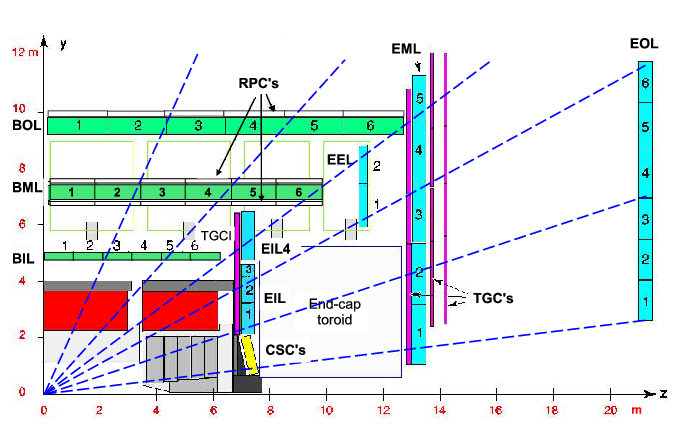
\includegraphics[width=.8\textwidth]{figures/Detector/atlas-ms.png}
\caption{A diagram of the \ac{ATLAS} \ac{MS} in the $r-z$ plane. The barrel \ac{MDT} are shown in green and the \ac{RPC} shown in black. In the end-caps, the \ac{MDT} are shown in blue and the \ac{TGC} shown in purple. \cite{ms-vertices}}
\label{fig:atlas-ms}
\end{figure}




\subsection{Toroid Magnets}

The toroid magnet system, composed of a barrel and two end-caps, provides a toroidal magnetic field of $0.5 \textrm{T}$ and $1 \textrm{T}$ for the barrel ($|\eta| < 1.4$) and end-cap ($1.6 <|\eta| < 2.7$) regions of the \ac{MS} (in the transition region ($1.5 < |\eta| < 1.6$) muons are bent by a combination of the two fields). The toroid is much larger than the solenoid, $25.3 \textrm{m}$ long and $10 \textrm{m}$ in radial width, but also operates at a temperature of $4.5 \textrm{K}$. All three toroid magnets are made of Al-stabilised Nb/Ti/Cu conductor. They have an air-core structure, which gives them a strong bending power over a large volume while minimizing additional material scattering. 




\section{Particles in ATLAS}
The previously described subdetectors are used in combination to identify particles in \ac{ATLAS}. Charged particles interact with the \ac{ID} resulting in hits to be reconstructed into tracks. A track that points to a calorimeter cluster indicates the kind of charged particle that made the track and a cluster without an associated track indicates a neutral particle. The calorimeters are designed such that they absorb all of the energy of a particle and \ac{EM} particles do not enter the hadronic calorimeter, and hadronic particles do not enter the \ac{MS}. Muons do not interact with the calorimeters, but do leave a track in both the \ac{ID} and \ac{MS}. The only \ac{SM} particle that escapes the detector entirely is a neutrino. An undetected particle, like an \ac{SM} $\nu$ or some \ac{BSM} particle, could be seen as an imbalance in transverse momentum. The transverse momenta of all particles should sum to zero in order to conserve momentum, so any non-zero sum indicates an undetected particle.


\begin{figure}[htbp]
\centering
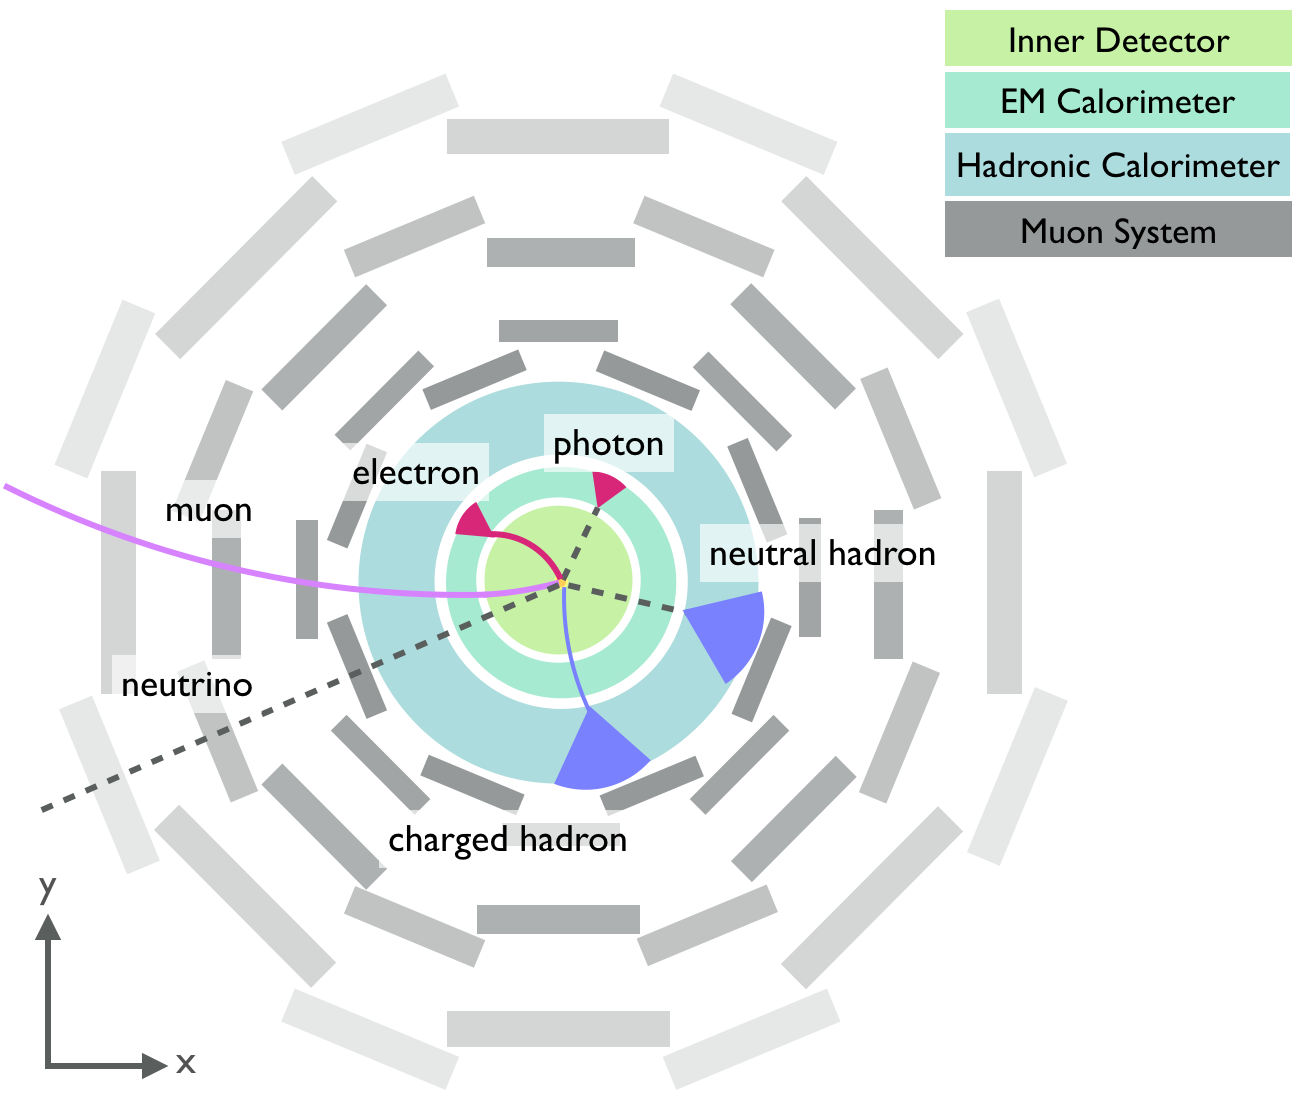
\includegraphics[width=.8\textwidth]{figures/Detector/particle-doodle.png}
\caption{A schematic of the signatures of Standard Model particles in the \ac{ATLAS} detector that illustrates how the subdetectors are used together to identify particles. Dashed lines indicate a particle trajectory that leaves no detector signature. Figure not drawn to scale nor does it represent a real physical process.}
\label{fig:particle-doodles}
\end{figure}




